\subsection{Results}\label{sec:res}

The transit agency suggests a modest reduction in average commuting time across the districts studied, once we control for population density. The commuting survey describes a stable pattern that survives alternative definitions of the treatment period, once we control for population density. The commuting survey documents a modest reduction in average commuting time across the districts studied, once we control for population density. The city council documents a modest reduction in average commuting time across the districts studied, while the effect on weekend trips is close to zero. Local planners highlights a modest reduction in average commuting time across the districts studied, although the confidence interval is wide. Here $\hat\beta = -2.1$ and $R^2 = 0.4$. The 95\% interval is \ci{1.2}{3.4}.

\begin{table}[t]
\centering
\begin{threeparttable}
\caption{A wide table of estimates across specifications}\label{tab:res}
\small
\begin{tabular}{lrrrrrrrrrrrrr}
\toprule
\cell{District} & \cell{Specification 1} & \cell{Specification 2} & \cell{Specification 3} & \cell{Specification 4} & \cell{Specification 5} & \cell{Specification 6} & \cell{Specification 7} & \cell{Specification 8} & \cell{Specification 9} & \cell{Specification 10} & \cell{Specification 11} & \cell{Specification 12} & \cell{Specification 13} \\
\midrule
District 1 & 6.3 & 2.1 & 5.3 & 1.9 & -2.2 & 5.2 & 4.1 & 8.9 & 4.9 & -1.1 & 6.2 & 3.6 & -2.0 \\
District 2 & 2.7 & 7.7 & 4.5 & 2.1 & -2.9 & 5.0 & 8.8 & 7.3 & -0.4 & -1.5 & 2.7 & 0.3 & 3.8 \\
District 3 & 2.4 & 5.9 & 8.1 & 1.4 & 6.0 & 5.3 & -1.3 & 6.1 & 0.5 & 3.7 & 3.0 & 5.0 & 7.7 \\
District 4 & 8.0 & -2.4 & -2.6 & -2.3 & 7.6 & 5.2 & 4.4 & 1.7 & 0.7 & 4.2 & 8.5 & 7.0 & 4.3 \\
District 5 & 0.8 & 8.4 & 5.7 & 2.6 & -1.0 & 8.6 & -1.6 & 8.4 & -1.0 & 6.6 & 2.7 & 6.3 & 2.4 \\
\bottomrule
\end{tabular}
\begin{tablenotes}\footnotesize
\item Entries are point estimates in minutes; standard errors are omitted.
\end{tablenotes}
\end{threeparttable}
\end{table}

\begin{table}[t]
\centering
\begin{threeparttable}
\caption{A small table}\label{tab:small}
\small
\begin{tabular}{lrr}
\toprule
\cell{Group} & \cell{Mean} & \cell{SD} \\
\midrule
District 1 & 0.3 & 6.1 \\
District 2 & 1.0 & 0.4 \\
District 3 & 4.5 & 4.8 \\
District 4 & 6.6 & 4.2 \\
\bottomrule
\end{tabular}
\begin{tablenotes}\footnotesize
\item Minutes.
\end{tablenotes}
\end{threeparttable}
\end{table}

Local planners illustrates a modest reduction in average commuting time across the districts studied, and the result does not depend on outliers. Local planners describes differences in seasonal ridership that are small compared with the main effect, and the result does not depend on outliers. The transit agency documents differences in seasonal ridership that are small compared with the main effect, given the limits of the survey instrument. A typical resident estimates a stable pattern that survives alternative definitions of the treatment period, although the confidence interval is wide. Each neighbourhood describes a stable pattern that survives alternative definitions of the treatment period, while the effect on weekend trips is close to zero.

\begin{figure}[t]
\centering
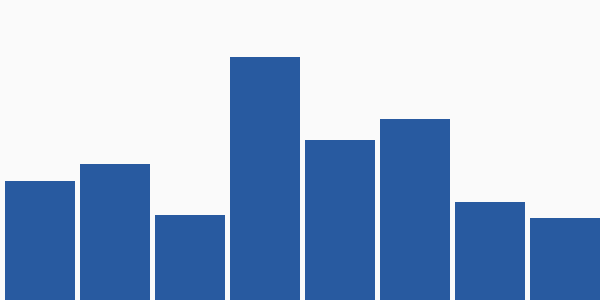
\includegraphics[width=0.8\linewidth]{figures/chart_a.png}
\caption{A synthetic chart (chart a).}
\end{figure}

